\vspace{-2pt}
\section{Experiments}
\label{sec:exp}
\vspace{-2pt}

% In this section, we aim to explore the following questions:
% \begin{itemize}[leftmargin=12pt]
% \item \textbf{Q1}: How well do current retrieval approaches perform on our benchmark datasets?
% \item \textbf{Q2}: What challenges are revealed by the experiments, and more importantly, what are the potential future directions for improvement?
% \end{itemize}


% \begin{itemize}[leftmargin=*]
%     \item \xhdr{Vector Similarity Search (ada-002)} 
%     ada-002 embeds the query and the concatenated textual and relational information of each candidate entity, then computes similarity scores between query and candidate embeddings. We use OpenAI's \texttt{text-embedding-ada-002} model for generating embeddings.

%     \item \xhdr{Multi-Vector Similarity Search (multi-ada-002)}
%     It represents each entity with multiple embeddings from chunks of its textual and relational information. We compute similarities between the query and chunk embeddings, then aggregate them by averaging the top-$k$ values as the final similarity.

%     \item \xhdr{Finetuned DPR} We finetunes query and document encoders using training query-answer pairs, optimizing with contrastive loss. Positive pairs are training questions and their ground truth answers; 20 hard negatives are top false positives from ada-002. We use \texttt{roberta-base} and finetune on the entire training split for each dataset.

%     \item \textbf{QAGNN}~\cite{qagnn}. 
%     QAGNN constructs a graph with nodes from candidate entities and entities mentioned in the question, including their neighbors for a rich context. It integrates semantic embeddings from a language model, jointly modeling relational and semantic information for retrieval.

%     \item \textbf{LLM Reranker}~\cite{abs-2306-04757, abs-2310-14122}. 
%     It improves the precision of the top-$k$ ada-002 results by reranking them with LLMs. We use GPT-4-turbo (\texttt{gpt-4-1106-preview}) and Claude3 (\texttt{claude-3-opus}), setting $k=20$ for synthesized and $k=10$ for human-generated queries. Given a query, the LLMs assign each candidate entity a satisfaction score from 0 to 1 based on their textual and relational information. 
%     We evaluate on a random 10\% sample of testing queries due to high retrieval costs.
%     \vspace{-5pt}
% \end{itemize}
\subsection{Baseline Retrieval Models and Evaluation Metrics}

We extensively evaluate five classes of retrieval models described below.
\vspace{-5pt}
\begin{itemize}[leftmargin=*]
    \vspace{-1pt}   
    \item \textbf{Sparse Retriever}: \textbf{BM25}~\cite{bm25} is a traditional yet powerful sparse retrieval method based on term frequency-inverse document frequency (TF-IDF). It computes relevance scores by considering the frequency of query terms in documents, adjusted for term rarity and document length.
    
    \vspace{-1pt}   
    \item \textbf{Small Dense Retrievers}: \textbf{DPR}~\cite{dpr}, \textbf{ANCE}~\cite{ance}, and \textbf{QAGNN}~\cite{qagnn}. These compact models generate dense embeddings for both queries and documents, computing retrieval scores based on embedding similarities. They serve as baselines for comparison with LLM-based dense retrievers.
    
    \vspace{-1pt}   
    \item \textbf{LLM-based Dense Retrievers}: \textbf{text-embedding-ada-002 (abbrev. ada-002)}~\cite{oai}, \textbf{voyage-large-2-instruct (abbrev. voyage-l2-instruct)}~\cite{voyage}, \textbf{LLM2Vec-Meta-Llama-3-8B-Instruct-mntp (abbrev. LLM2Vec)}~\cite{llm2vec}, and \textbf{GritLM-7b}~\cite{GritLM}. These models leverage LLMs to generate dense embeddings that are more contextually expressive.
    
    \vspace{-1pt}   
    \item \textbf{Multivector Retrievers}: \textbf{multi-ada-002}~\cite{oai} and \textbf{ColBERTv2}~\cite{ColBERTv2}. Beyond ada-002 which represents a document as an embedding, \textbf{multi-ada-002} splits each document into overlapping chunks and embeds them using the same encoder as the query. Similarity scores between the query and chunks are aggregated using the average of the top-3 similarities, which we found to perform best. \textbf{ColBERTv2} represents each document as multiple token-level embeddings for fine-grained matching, capturing richer semantic information.
    
    \vspace{-1pt}   
    \item \textbf{LLM Rerankers}: \textbf{Claude3} and \textbf{GPT-4} rerankers~\cite{abs-2306-04757, abs-2310-14122}. These models improve the precision of top-$k$ ada-002 results by reranking them using large language models. We employ GPT-4-turbo (\texttt{gpt-4-1106-preview}) and Claude3 (\texttt{claude-3-opus}), setting $k=20$ for synthesized queries and $k=10$ for human-generated queries. Given a query, the LLMs assign a satisfaction score from 0 to 1 to each candidate entity based on textual and relational information. Due to high computational costs, we evaluate these rerankers on a random 10\% sample of test queries.
\end{itemize}

The performance of these models are measured using standard retrieval metrics below.

% We use metrics including Hit@1, Hit@5, Mean Reciprocal Rank (MRR), and Recall@20. See Appendix~\ref{app:metrics} for details.

% \subsection{Evaluation Metrics}
% \label{app:metrics}

% We use the following metrics to holistically evaluate the model performance.

\vspace{-5pt}
\begin{itemize}[leftmargin=*]

    \vspace{-1pt}   
    \item \textbf{Hit@$k$} assesses whether the correct item is among the top-$k$ results from the model. We used $k=1$ and $k=5$ for evaluation. At $k=1$, it evaluates the accuracy of the top recommendation; at $k=5$, it examines the model's precision in a wider recommendation set.  
    % It's a straightforward yet effective way to measure the immediate relevance of answers.

    \vspace{-1pt}   
    \item \textbf{Recall@$k$} measures the proportion of relevant items in the top-$k$ results. For synthesized queries, $k=20$ is used, as the answer length of all of the queries in our benchmarks are equal or smaller then $20$. 
    % For human-generated queries, Recall@20 is not reported as the number of responses in the human-generated subset may exceed 20. 
    This metric offers insight into the model's ability to identify all relevant items, particularly in scenarios where missing any could be critical. 

    \vspace{-1pt}   
    \item \textbf{Mean Reciprocal Rank (MRR)} is a statistic for evaluating the average effectiveness of a predictive model. It calculates the reciprocal of the rank at which the first relevant item appears in the list of predictions. 
    % MRR is particularly useful for understanding the model's performance at presenting the correct item at an early stage, without the need for a predefined $k$. 
    This metric emphasizes the importance of the rank of the first correct answer, which is crucial in many practical applications where the first correct answer is often the most impactful.
\end{itemize}

\subsection{Results and Analysis}
\vspace{-2pt}

% \begin{table}[htbp]
%     \centering
%     \resizebox{1.0\textwidth}{!}{
%     \begin{tabular}{l|cccc|cccc|cccc}
%         \toprule
%         & \multicolumn{4}{c|}{\amazont} & \multicolumn{4}{c|}{\magt} & \multicolumn{4}{c}{\primekgt} \\
%         & \textbf{\small Hit@1} & \textbf{\small Hit@5} & \textbf{\small Recall@20} & \textbf{\small MRR} & \textbf{\small Hit@1} & \textbf{\small Hit@5} & \textbf{\small Recall@20} & \textbf{\small MRR} & \textbf{\small Hit@1} & \textbf{\small Hit@5} & \textbf{\small Recall@20} & \textbf{\small MRR}  \\
%         \midrule
%         % \textbf{RAG-Base} &0.0673& 0.1561 & 0.1233 &0.1373  &0.0349&0.0513 & 0.0555& 0.0369& 0.0324 & 0.0834& 0.1008 & 0.0588 \\
%         \textbf{Dense Retriever (\texttt{roberta})}        & 0.1529 & 0.4793& 0.4449&0.3020&&&\\
%         \textbf{QAGNN (\texttt{roberta})}        &&&&\\
%         \textbf{VSS (\texttt{ada-002})}        & 0.3916 & 0.6273 & 0.5329 & 0.5035 & 0.2908 & 0.4961 & 0.4836 & 0.3862 & 0.1263 & 0.3149 & 0.3600 & 0.2141\\
%         \textbf{MultiVSS (\texttt{ada-002})} & 0.4007 & 0.6498 & 0.5512 & 0.5155 & 0.2592 & 0.5043 & 0.5080 & 0.3694 & 0.1510 & 0.3356 & 0.3805 & 0.2349\\
%         % \textbf{RAG-FT} &0.2026 & 0.3037 & 0.3969  & 0.2340  &0.0361 &0.0482 & 0.0627&0.0442& 0.0370 &0.0867 & 0.1359 & 0.0618\\
%         \textbf{VSS+Claude Reranker}   & 0.4266 & 0.6746 & 0.5376 & 0.5329 & 0.3202& 0.5334&  0.4834& 0.4129& 0.1611 & 0.3582 & 0.3598 & 0.2466\\
%         \textbf{VSS+GPT4 Reranker}   & 0.4479 & 0.7117 & 0.5535 & 0.5569 &0.4090 &0.5818 &0.4860 & 0.4900& 0.1828 & 0.3728&0.3405 & 0.2655\\
%         \bottomrule
%     \end{tabular}
%         }
%     \label{tab:results}
%     \caption{Main experimental results. Last row shows the relative improvements over the best metric value among the baselines.}
% \end{table}


% \begin{table}[htbp]
%     \centering
%     \resizebox{1.0\textwidth}{!}{
%     \begin{tabular}{l|cccc|cccc|cccc}
%         \toprule
%         & \multicolumn{4}{c|}{\amazont} & \multicolumn{4}{c|}{\magt} & \multicolumn{4}{c}{\primekgt} \\
%         & \textbf{\small Hit@1} & \textbf{\small Hit@5} & \textbf{\small Recall@20} & \textbf{\small MRR} & \textbf{\small Hit@1} & \textbf{\small Hit@5} & \textbf{\small Recall@20} & \textbf{\small MRR} & \textbf{\small Hit@1} & \textbf{\small Hit@5} & \textbf{\small Recall@20} & \textbf{\small MRR}  \\
%         \midrule
%         \textbf{Dense Retriever (\texttt{roberta})}        & 0.1529 & 0.4793& 0.4449&0.3020&&&\\
%         \textbf{QAGNN (\texttt{roberta})}        &&&&\\
%         \textbf{VSS (\texttt{ada-002})}        & 0.3916 & 0.6273 & 0.5329 & 0.5035 & 0.2908 & 0.4961 & 0.4836 & 0.3862 & 0.1263 & 0.3149 & 0.3600 & 0.2141\\
%         \textbf{MultiVSS (\texttt{ada-002})} & 0.4007 & 0.6498 & 0.5512 & 0.5155 & 0.2592 & 0.5043 & 0.5080 & 0.3694 & 0.1510 & 0.3356 & 0.3805 & 0.2349\\
%         \textbf{VSS+Claude Reranker}   & 0.4266 & 0.6746 & 0.5376 & 0.5329 & 0.3202& 0.5334&  0.4834& 0.4129& 0.1611 & 0.3582 & 0.3598 & 0.2466\\
%         \textbf{VSS+GPT4 Reranker}   & 0.4479 & 0.7117 & 0.5535 & 0.5569 &0.4090 &0.5818 &0.4860 & 0.4900& 0.1828 & 0.3728&0.3405 & 0.2655\\
%         \bottomrule
%     \end{tabular}
%         }
%     \label{tab:results}
%     \caption{Main experimental results. Last row shows the relative improvements over the best metric value among the baselines.}
% \end{table}

% submit
% \begin{table}[t]
%     \centering
%     \vspace{-10pt}
%     \caption{\textbf{Testing results on \benchmarkt-Syn(thesized).} (*) indicates partial evaluation (on random 10\% of the test queries) due to the high latency and cost of the methods. }
%     \resizebox{0.9\textwidth}{!}{
%     \begin{tabular}{l|lcccccc}
%         \toprule
%         && \textbf{\small Dense Retriever} & \textbf{\small QAGNN } & \textbf{\small VSS} & \textbf{\small MultiVSS} & \textbf{*\small Claude3} & \textbf{*\small GPT4} \\
%         &&{\small\texttt{(roberta)}} &{\small\texttt{(roberta)}}&{\small \texttt{(ada-002)}}&{\small \texttt{(ada-002)}}& \textbf{\small Reranker} & \textbf{\small Reranker}\\
%         \midrule
%         \multirow{4}{*}{\textbf{\small \amazont}}&Hit@1    & 0.1529 & 0.2656 & 0.3916 & 0.4007 & \textbf{0.4549} & 0.4479 \\
%         &Hit@5    & 0.4793 & 0.5001 & 0.6273 & 0.6498 & 0.7113 & \textbf{0.7117} \\
%         &Recall@20& 0.4449 & 0.5205 & 0.5329 & 0.5512 & 0.5377 & \textbf{0.5535} \\
%         &MRR      & 0.3020 & 0.3775 & 0.5035 & 0.5155 & \textbf{0.5591} & 0.5569 \\
%         \midrule
%         \multirow{4}{*}{\textbf{\small\magt}}&Hit@1    &0.1051 & 0.1288 & 0.2908 & 0.2592 & 0.3654 & \textbf{0.4090} \\
%         &Hit@5    &0.3523 & 0.3901 & 0.4961 & 0.5043 & 0.5317 & \textbf{0.5818} \\
%         &Recall@20& 0.4211 & 0.4697 & 0.4836 & \textbf{0.5080} & 0.4836 & 0.4860 \\
%         &MRR      & 0.2134 & 0.2912 & 0.3862 & 0.3694 & 0.4415 & \textbf{0.4900} \\
%         \midrule
%         \multirow{4}{*}{\textbf{\small\primekgt}} &Hit@1    &0.0446 & 0.0885 & 0.1263 & 0.1510 & 0.1779 &\textbf{ 0.1828} \\
%         &Hit@5    &0.2185 & 0.2135 & 0.3149 & 0.3356 & 0.3690 & \textbf{0.3728} \\
%         &Recall@20 & 0.3013 & 0.2963 & 0.3600 & \textbf{0.3805} & 0.3557 & 0.3405 \\
%         &MRR &0.1238 & 0.1473 & 0.2141 & 0.2349 & 0.2627 & \textbf{0.2655} \\
%         \bottomrule
%     \end{tabular}
%     }
%     \vspace{-15pt}
%     \label{tab:results}
% \end{table}

\begin{table}[t]
    \centering
    \vspace{-10pt}
    \caption{Testing results on \benchmarkt-Syn(thesized).}
    \resizebox{1.0\textwidth}{!}{
    \begin{tabular}{r|rrrr|rrrr|rrrr}
        \toprule
        & \multicolumn{4}{c|}{\amazont} & \multicolumn{4}{c|}{\magt} & \multicolumn{4}{c}{\primekgt} \\
         & Hit@1 & Hit@5 & R@20 & MRR & Hit@1 & Hit@5 & R@20 & MRR & Hit@1 & Hit@5 & R@20 & MRR \\
        \hline
        \rowcolor{cyan!10} \multicolumn{13}{c}{\textbf{Full Testing Dataset}} \\
        \hline
        BM25 & 44.94 & \textbf{67.42} & 53.77 & 55.30 & 25.85 & 45.25 & 45.69 & 34.91 & 12.75 & 27.92 & 31.25 & 19.84 \\
        DPR (roberta) & 15.29 & 47.93 & 44.49 & 30.20 & 10.51 & 35.23 & 42.11 & 21.34 & 4.46 & 21.85 & 30.13 & 12.38 \\
        ANCE (roberta) & 30.96 & 51.06 & 41.95 & 40.66 & 21.96 & 36.50 & 35.32 & 29.14 & 6.53 & 15.67 & 16.52 & 11.05 \\
        
        QAGNN (roberta) & 26.56 & 50.01 & 52.05 & 37.75 & 12.88 & 39.01 & 46.97 & 29.12 & 8.85 & 21.35 & 29.63 & 14.73 \\
        ada-002 & 39.16 & 62.73 & 53.29 & 50.35 & 29.08 & 49.61 & 48.36 & 38.62 & 12.63 & 31.49 & 36.00 & 21.41 \\
        % VSS (oai-3-large) & - & - & - & - & 38.04 & 61.50 & 59.03 & 48.95 & 16.32 & 38.52 & 45.51 & 26.63 \\
        voyage-l2-instruct & 40.93 & 64.37 & 54.28 & 51.60 & 30.06 &  50.58 & \textbf{50.49} & 39.66 & 10.85 & 30.23 & 37.83 & 19.99 \\ 
        LLM2Vec & 21.74 & 41.65 & 33.22 & 31.47 & 18.01 & 34.85 & 35.46 & 26.10 & 10.10 & 22.49 & 26.34 & 16.12 \\
        GritLM-7b & 42.08 & 66.87 & \textbf{56.52} & 53.46 & \textbf{37.90} & \textbf{56.74} & 46.40 & \textbf{47.25} & \textbf{15.57} & 33.42 & \textbf{39.09} & \textbf{24.11} \\
        multi-ada-002 & 40.07 & 64.98 & 55.12 & 51.55 & 25.92 & 50.43 & 50.80 & 36.94 & 15.10 & \textbf{33.56} & 38.05 & 23.49 \\
        ColBERTv2 & \textbf{46.10} & 66.02 & 53.44 & \textbf{55.51} & 31.18 & 46.42 & 43.94 & 38.39 & 11.75 & 23.85 & 25.04 & 17.39 \\
        \hline
        \rowcolor{green!8} \multicolumn{13}{c}{\textbf{Random 10\% Sample}} \\
        \hline
        BM25 & 42.68 & 67.07 & 54.48 & 54.02 & 27.81 & 45.48 & 44.59 & 35.97 & 13.93 & 31.07 & 32.84 & 21.68 \\
        DPR (roberta) & 16.46 & 50.00 & 42.15 & 30.20 & 11.65 & 36.84 & 42.30 & 21.82 & 5.00 & 23.57 & 30.50 & 13.50 \\
        ANCE (roberta) & 30.09 & 49.27 & 41.91 & 39.30 & 22.89 & 37.26 &44.16 & 30.00 & 6.78 & 16.15 & 17.07 & 11.42 \\
        QAGNN (roberta) & 25.00 & 48.17 & 51.65 & 36.87 & 12.03 & 37.97 & 47.98 & 28.70 & 7.14 & 17.14 & 32.95 & 16.27 \\
        ada-002 & 39.02 & 64.02 & 49.30 & 50.32 & 28.20 & 52.63 & 49.25 & 38.55 & 15.36 & 31.07 & 37.88 & 23.50 \\
        voyage-l2-instruct & 43.29 & 67.68 & 56.04 & 54.20 & 34.59 & 50.75 & 50.75 & 42.90 & 12.14 & 31.42 & 37.34 & 21.23 \\
        LLM2Vec & 18.90 & 37.80 & 34.73 & 28.76 & 19.17 & 33.46 & 29.85 & 26.06 & 9.29 & 20.7 & 25.54 & 15.00 \\
        GritLM-7b & 43.29 & \textbf{71.34} & \textbf{56.14} & 55.07 & 38.35 & \textbf{58.64} & 46.38 & 48.25 & 16.79 & 34.29 & 41.11 & 24.99 \\
        % VSS (oai-3-large) & - & - & - & - & - & - & - & - & - & - & - & - \\
        multi-ada-002 & 40.85 & 62.80 & 52.47 & 51.54 & 25.56 & 50.37 & \textbf{53.03} & 36.82 & 15.36 & 32.86 & \textbf{40.99} & 23.70 \\
        ColBERTv2 & 44.31 & 65.24 & 51.00 & 55.07 & 31.58 & 47.36 & 45.72 & 38.98 & 15.00 & 26.07 & 27.78 & 19.98 \\
        Claude3 Reranker & \textbf{45.49} & 71.13 & 53.77 & \textbf{55.91} & 36.54 & 53.17 & 48.36 & 44.15 & 17.79 & 36.90 & 35.57 & 26.27 \\
        GPT4 Reranker & 44.79 & 71.17 & 55.35 & 55.69 & \textbf{40.90} & 58.18 & 48.60 & \textbf{49.00} & \textbf{18.28} & \textbf{37.28} & 34.05 & \textbf{26.55} \\
        \bottomrule
    \end{tabular}
    }
    \label{tab:results}
\end{table}


% \begin{table}[h]
%     \centering
%     \vspace{-15pt}
%     \caption{Testing results on \benchmarkt-Human(-Generated).}
%     \resizebox{0.85\textwidth}{!}{
%     \begin{tabular}{l|lcccc}
%         \toprule
%         & & \textbf{\small VSS} & \textbf{\small MultiVSS} & \textbf{\small Claude3} & \textbf{\small GPT4} \\
%         & & {\small \texttt{(ada-002)}}&{\small \texttt{(ada-002)}}& \textbf{\small Reranker} & \textbf{\small Reranker}\\
%         \midrule
%         \multirow{3}{*}{\textbf{\small \amazont}}
%         &Hit@1    & 0.3950 & 0.4691 & \textbf{0.5602} & 0.5432 \\
%         &Hit@5    & 0.6419 & \textbf{0.7284} & \textbf{0.7284} & \textbf{0.7284}\\
%         &Recall@20    & 0.3546 & \textbf{0.4022} & 0.3546 & 0.3546 \\\
%         &MRR      & 0.5265 & 0.5874 & \textbf{0.6439} & 0.6274\\
%         \midrule
%         \multirow{3}{*}{\textbf{\small\magt}}
%         &Hit@1    & 0.2857 & 0.2381 & \textbf{0.3810} & 0.3690 \\
%         &Hit@5    & 0.4167 & 0.4167 & \textbf{0.4643} & 0.4523\\
%         % &Recall@20& & & & \\
%         &Recall@20    & 0.3595 & \textbf{0.3985} & 0.3595 & 0.3595\\
%         &MRR      & 0.3581 & 0.3143 & \textbf{0.4243} & 0.4031\\
%         \midrule
%         \multirow{3}{*}{\textbf{\small\primekgt}} 
%         &Hit@1    & 0.2120 & 0.2567 & \textbf{0.2844} & \textbf{0.2844}\\
%         &Hit@5    & 0.4037 & 0.4037 & 0.4771 & \textbf{0.4863} \\
%         &Recall@20    & 0.4383 & \textbf{0.4979} & 0.4383  & 0.4383 \\
%         % &Recall@20 & & & & \\
%         &MRR      & 0.2984 & 0.3377 & \textbf{0.3623} & 0.3617 \\
%         \bottomrule
%     \end{tabular}
%     }
%     \label{tab:results-human}
% \end{table}

\begin{table}[t]
    \centering
    \vspace{-10pt}
    \caption{Testing results on \benchmarkt-Human(-Generated).}
    \resizebox{1.0\textwidth}{!}{
    \begin{tabular}{r|rrrr|rrrr|rrrr}
        \toprule
        & \multicolumn{4}{c|}{\textbf{\amazont}} & \multicolumn{4}{c|}{\textbf{\magt}} & \multicolumn{4}{c}{\textbf{\primekgt}} \\
        Method & Hit@1 & Hit@5 & R@20 & MRR & Hit@1 & Hit@5 & R@20 & MRR & Hit@1 & Hit@5 & R@20 & MRR \\
        \midrule
        BM25 & 27.16 & 51.85 & 29.23 & 18.79 & 32.14 & 41.67 & 32.46 & 37.42 & 22.45 & 41.84 & 42.32 & 30.37 \\
        DPR (roberta) & 16.05 & 39.51 & 15.23 & 27.21 & 4.72 & 9.52 & 25.00 & 7.90 & 2.04 & 9.18 & 10.69 & 7.05 \\
        ANCE (roberta) &25.93 & 54.32 & 23.69 & 37.12 & 25.00 & 30.95 & 27.24 & 27.98 & 7.14 & 13.27 & 11.72 & 10.07 \\
        QAGNN (roberta) & 22.22 & 49.38 & 21.54 & 31.33 & 20.24 & 26.19 & 28.76 & 25.53 & 6.12 & 13.27 & 17.62 & 9.39 \\
        ada-002 & 39.50 & 64.19 & 35.46 & 52.65 & 28.57 & 41.67 & 35.95 & 35.81 & 17.35 & 34.69 & 41.09 & 26.35 \\
        voyage-l2-instruct & 35.80 & 62.96 & 33.01 & 47.84 & 22.62 & 36.90 & 32.44 & 29.68 & 16.33 & 32.65 & 39.01 & 24.33 \\
        LLM2Vec & 29.63 & 46.91 & 21.21 & 38.61 & 16.67 & 28.57 & 21.74 & 21.59 & 9.18 & 21.43 & 26.77 & 15.24 \\
        GritLM-7b & 40.74 & 71.60 & 36.30 & 53.21 & 34.52 & 44.04 & 34.57 & 38.72 & 25.51 & 41.84 & \textbf{48.10} & 34.28 \\ 
        multi-ada-002 & 46.91 & 72.84 & \textbf{40.22} & 58.74 & 23.81 & 41.67 & \textbf{39.85} & 31.43 & 24.49 & 39.80 & 47.21 & 32.98 \\
        ColBERTv2 & 33.33 & 55.56 & 29.03 & 43.77 & 33.33 & 36.90 & 30.50 & 35.97 & 15.31 & 26.53 & 25.56 & 19.67 \\
        Claude3 Reranker & \textbf{53.09} & 74.07 & 35.46 & \textbf{62.11} & \textbf{38.10} & 45.24 & 35.95 & \textbf{42.00} & \textbf{28.57} & \textbf{46.94} & 41.61 & \textbf{36.32} \\
        GPT4 Reranker & 50.62 & \textbf{75.31} & 35.46 & 61.06 & 36.90 & \textbf{46.43} & 35.95 & 40.65 & \textbf{28.57} & 44.90 & 41.61 & 34.82 \\
        \bottomrule
    \end{tabular}
    }
    \label{tab:results-human}
    \vspace{-10pt}
\end{table}



\textbf{Results on synthesized queries.} 
Table~\ref{tab:results} presents the results on both the full synthesized test sets and random 10\% samples from these sets. In both cases, \textbf{BM25}, despite its simplicity, proves to be a strong baseline, outperforming the dense retrieval models such as \textbf{ANCE}. We observe that finetuned \textbf{DPR} and \textbf{QAGNN}, exhibit insufficient performance. This underperformance is likely due to their relatively small model sizes and the risk of overfitting during training. These issues present challenges in effectively training the models on SKBs, where the entity documents can be hard to differentiate without capturing detailed information.

Among the larger models, \textbf{ada-002} benefits from superior pretrained embeddings and significantly outperforms \textbf{LLM2Vec} by a large margin. \textbf{GritLM-7b} delivers excellent performance, surpassing the ada-002 model overall. In contrast, LLM2Vec underperforms due to its limited context length, which is insufficient for encoding the lengthy documents in the SKBs. For multivector retrievers, we found that \textbf{multi-ada-002} generally outperforms ada-002, indicating that using multiple vectors per document enhances retrieval effectiveness. Similarly, fine-grained representation allows \textbf{ColBERTv2} to capture subtle semantic nuances between queries and documents, leading to largely improved retrieval accuracy. 

However, both GritLM-7b and ColBERTv2 generally underperform compared to the rerankers on the random split, especially in terms of Hit@k metrics. This suggests that while these dense retriever models effectively capture semantic information, they may not fully grasp the nuanced relevance judgments required for top-tier retrieval performance. The rerankers, utilizing powerful LLMs like \textbf{GPT-4 (gpt-4-1106-preview)} and \textbf{Claude3 (claude-3-opus)}, excel by re-evaluating the top candidates and assigning satisfaction scores based on a deeper understanding of the query and document content. This process allows them to better discern subtle contextual cues and relational information that dense retrievers might overlook. Consequently, LLM rerankers enhance retrieval precision at the top ranks.

Finally, regardless of the higher computational costs of the rerankers, their performance remains suboptimal. For instance, the Hit@1 scores for the GPT-4 reranker are only about 18\% on \primekgt and 41\% on \magt, indicating that the top-ranked answers are frequently incorrect. Similarly, the Recall@20 metrics are below 60\% across all datasets, with the GPT-4 reranker achieving Recall@20 scores of 55\% on \amazont, 49\% on \magt, and 34\% on \primekgt. This suggests that the ranking results miss a significant portion of relevant answers. The MRR scores are also relatively low, especially for \primekgt, where the GPT-4 reranker attains an MRR of only around 27\%. 

The insufficient performances may be attributed to the complexity and diversity of queries in SKBs, where nuanced understanding and detailed contextual information are crucial.
These findings highlight significant room for improvement in the ranking process.


\xhdr{Results on human-generated dataset}  
Table~\ref{tab:results-human} presents the testing results on the human-generated datasets. For example, the rerankers consistently outperform others, showing their reasoning and context understanding ability. Compared to the synthesized datasets, the performance on human-generated queries is generally higher for most models, but the overall trends remain consistent. This indicates that synthesized datasets may be more challenging, highlighting the complexity of the tasks on our synthesized queries. 

Another interesting observation is that the performance of the rerankers is particularly strong on human-generated queries, which may contain more nuanced language and diverse expressions. This suggests that rerankers excel in interpreting and leveraging the richness of human language to improve retrieval accuracy.



\begin{table}[t]
    \centering
    \caption{Latency (s) of the retrieval systems on \benchmarkt. }
    \resizebox{0.9\textwidth}{!}{
    \begin{tabular}{l|cccccc}
        \toprule
        &\textbf{\small DPR} & \textbf{\small QAGNN } & 
        \textbf{\small ada-002} & \textbf{\small multi-ada-002} & \textbf{\small Claude3 Reranker} & \textbf{\small GPT4 Reranker} \\
        \midrule
        \textbf{\amazont} & 2.34 & 2.32 &5.71 &4.87 & 27.24&24.76 \\
        \textbf{\magt} & 0.94 &1.35 &2.25 &3.14 &22.60 & 23.43 \\
        \textbf{\primekgt} & 0.92 & 1.29 &0.54 &0.90 &29.14 &26.97 \\
        \midrule 
        \textbf{Average} & 1.40  & 1.65 &2.83 &2.97 &26.33 &25.05 \\
        \bottomrule
    \end{tabular}
    }
    \label{tab:latency}
    \vspace{-10pt}
\end{table}

% On the other hand, this suggests the complexities of 
% for our benchmark and demonstrates the value of a double-checking process due to the complexities of our text and relational data requirements.


\begin{figure}[t]
    \centering
    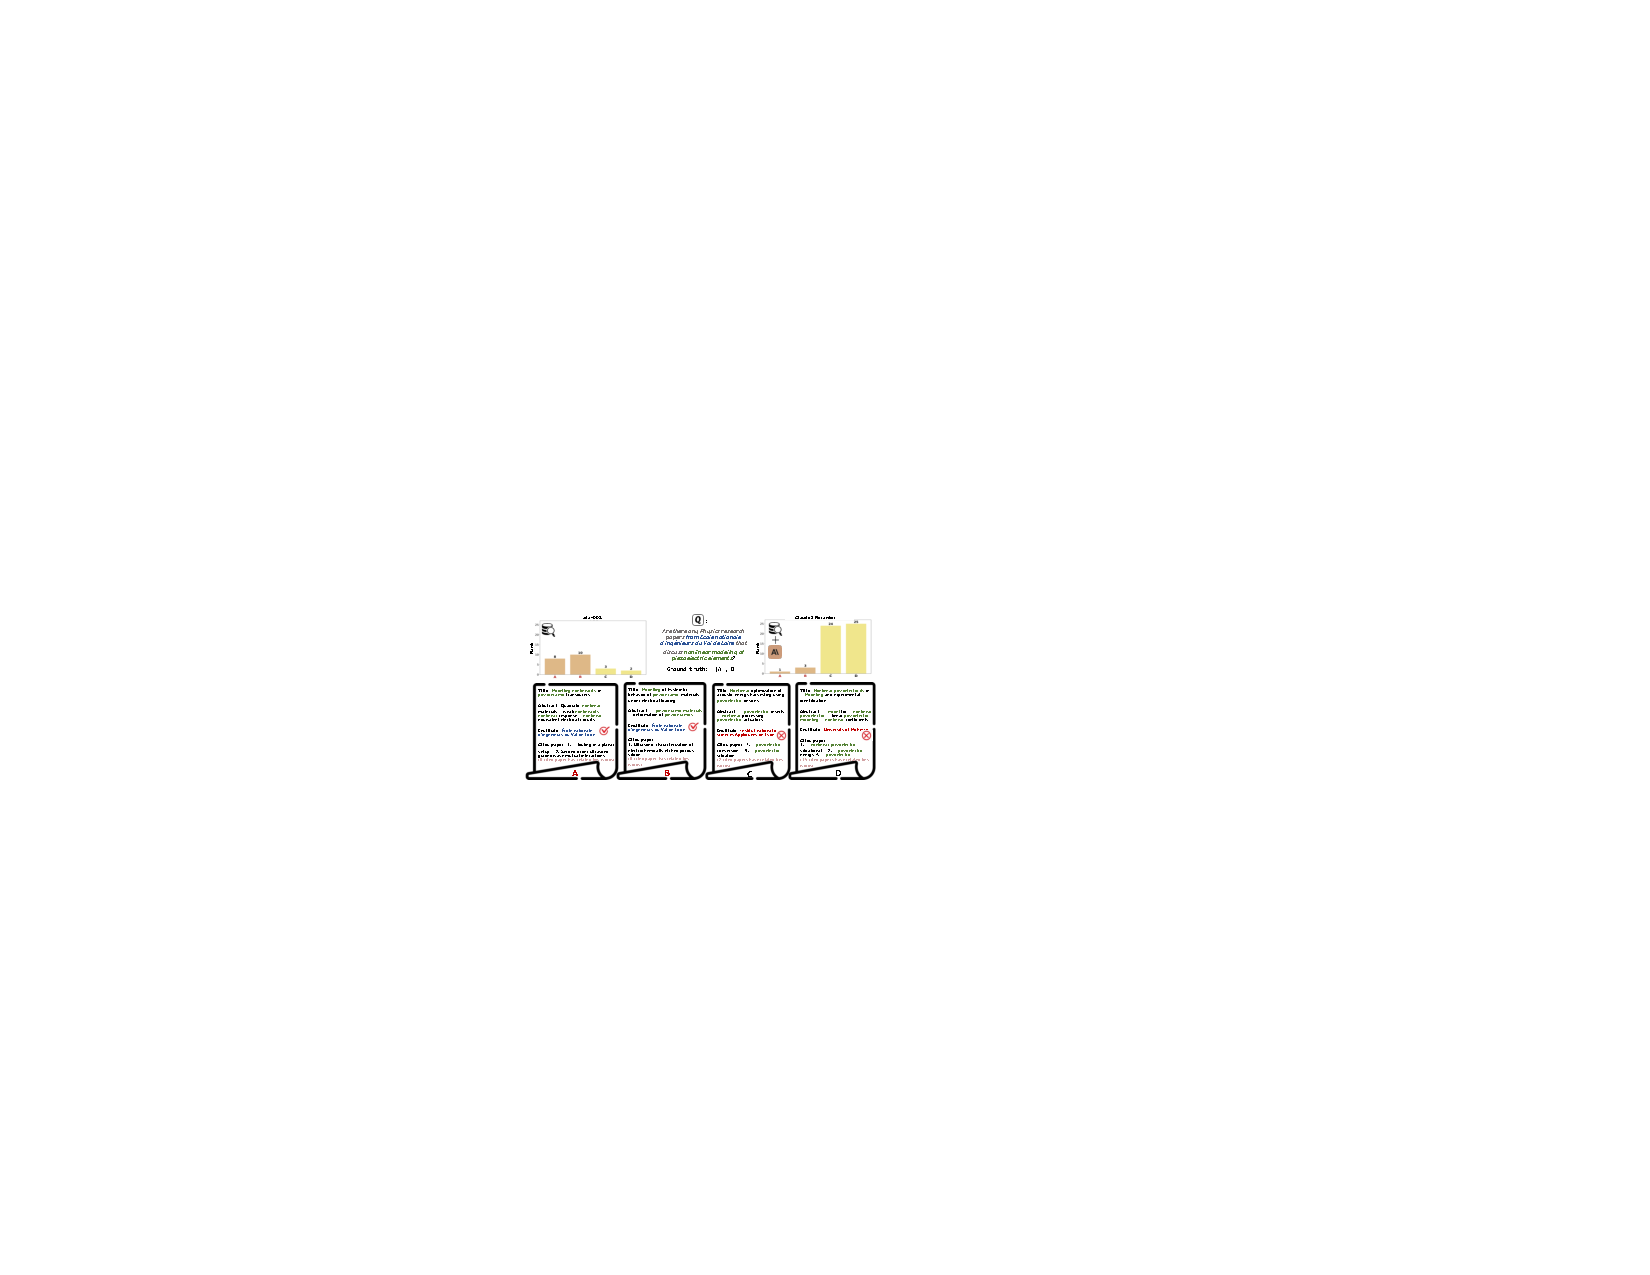
\includegraphics[width=1\textwidth]{figs/case_updated}
    \caption{
    A case study on \magh shows that ada-002 overranks non-ground truth papers $C$ and $D$ due to repeated keywords in the relational information ``cites paper''. After reranking with Claude3, it correctly prioritizes ground truth papers $A$ and $B$ with accurate reasoning and analysis.}
    \vspace{-10pt}
    \label{fig:case}
\end{figure}

\xhdr{Retrieval latency} Latency is crucial for practical retrieval systems, as users expect quick responses. As shown in Table~\ref{tab:latency}, we evaluated the latency of various models using a single NVIDIA A100-SXM4-80GB GPU. We observed that the DPR and QAGNN models exhibit lower average latency, making them suitable for time-sensitive applications. In contrast, the ada-002 and multi-ada-002 models have moderate latency due to multiple API calls. However, when combined with LLM rerankers, the latency increases significantly due to the computational demands of these large models. Therefore, it is important to balance accuracy and latency, especially for complex queries that require advanced reasoning capabilities. 


\xhdr{Case study} 
To highlight the importance of reasoning ability for achieving good performance on our benchmark, we present a case study in Figure~\ref{fig:case}, comparing the ada-002 model with the Claude3 Reranker. In this example, the query requests papers from a specific institution on a particular topic. The ada-002 model fails to address the relational aspect of the query because it embeds entire documents without detailed analysis. This leads to high relevance scores for irrelevant papers that frequently mention keywords like "nonlinear modeling" and "piezoelectric elements" but do not satisfy the relational requirement. In contrast, the LLM reranker significantly improves the results by reasoning about the relationship between the query and each paper, resulting in scores that more accurately reflect relevance. This underscores the need for reasoning ability to grasp query complexities. 

